% !TEX root=talk.tex

\section{Document Types}

\begin{frame}[fragile]
\frametitle{Article -- The Basic Document}

\begin{columns}
\begin{column}{.4\textwidth}
\begin{beamerboxesrounded}[width=\linewidth]{}
\begin{lstlisting}[moretexcs={chapter,subsection,maketitle}, basicstyle={\ttfamily}, emph={article}]
\documentclass{article}
\author{...}
\title{...}

\begin{document}
\maketitle
\section{...}
...
\subsection{...}
\end{document}
\end{lstlisting}
\end{beamerboxesrounded}
\end{column}
\begin{column}{.58\textwidth}
\centering
\fcolorbox{black}{white}{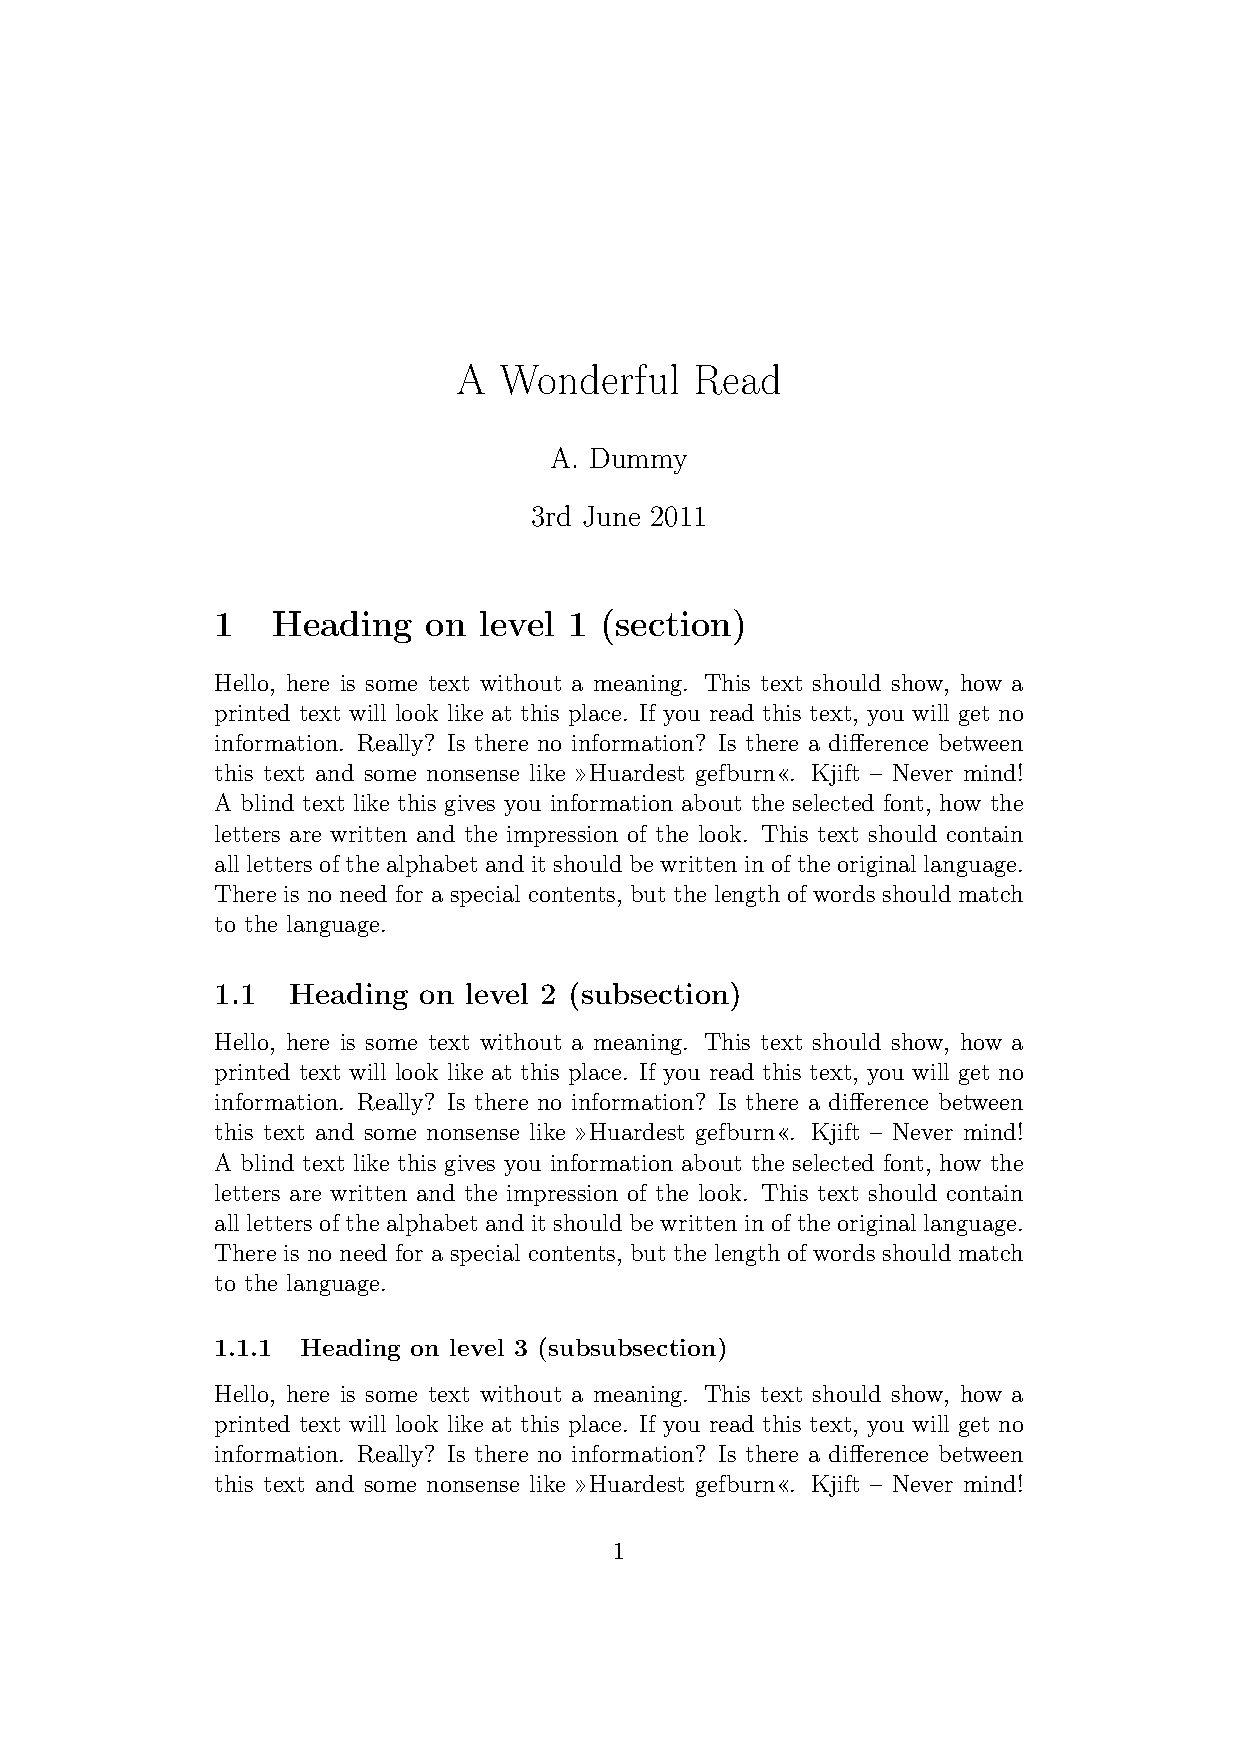
\includegraphics[width=.4\linewidth,page=1]{examples/basicarticle}}
\fcolorbox{black}{white}{\includegraphics[width=.4\linewidth,page=2]{examples/basicarticle}}
\fcolorbox{black}{white}{\includegraphics[width=.4\linewidth,page=3]{examples/basicarticle}}
\fcolorbox{black}{white}{\includegraphics[width=.4\linewidth,page=4]{examples/basicarticle}}
\end{column}
\end{columns}
\end{frame}




\begin{frame}[fragile]
\lstset{basicstyle=\ttfamily}
\frametitle{Some Features of \LaTeX}
\begin{itemize}
\item<+> Automatic generation of \structure{cross-referencing labels}:\\
\lstinline|\section{Introduction}\label{sec:intro}|\\
\lstinline|... We saw in section \ref{sec:intro}...|
\item<+> Automatic generation of \structure{lists}:\\
\lstinline[texcs={tableofcontents}]|\tableofcontents|, \lstinline[texcs={listoffigures}]|\listoffigures|,  \lstinline[texcs={listoftables}]|\listoftables|
\item<+> Automatic generation of \structure{bibliographies} and \structure{indices}:\\
\lstinline|\cite{Knuth:1976}...\bibliography{references.bib}|\\
\lstinline[moretexcs={printindex}]|...the Linux kernel\index{Linux!kernel}... \printindex|\\
\item<+> Fully \structure{hyperlinked} \textsmaller{PDF} with bookmarks: \lstinline|\usepackage{hyperref}|
\item<+> Inclusion of selected pages from other \textsmaller{PDF}s\\(while inserting new page headers/footers!)\\
\lstset{basicstyle=\ttfamily\footnotesize,moretexcs={includepdf}}
\lstinline|\usepackage{pdfpages}|\\
\lstinline|\includepdf[pages={1,3-5,8},pagecommand=\thispagestyle{plain}]{file.pdf}|
\item<+> Quick \structure{language-switching} with \texttt{babel}
\end{itemize}
\end{frame}


\begin{frame}[fragile]
\frametitle{Your Final Year Project}

\bigskip
\bigskip

A template for a university thesis.

\vskip.5em

\begin{center}
\fcolorbox{black}{white}{%
  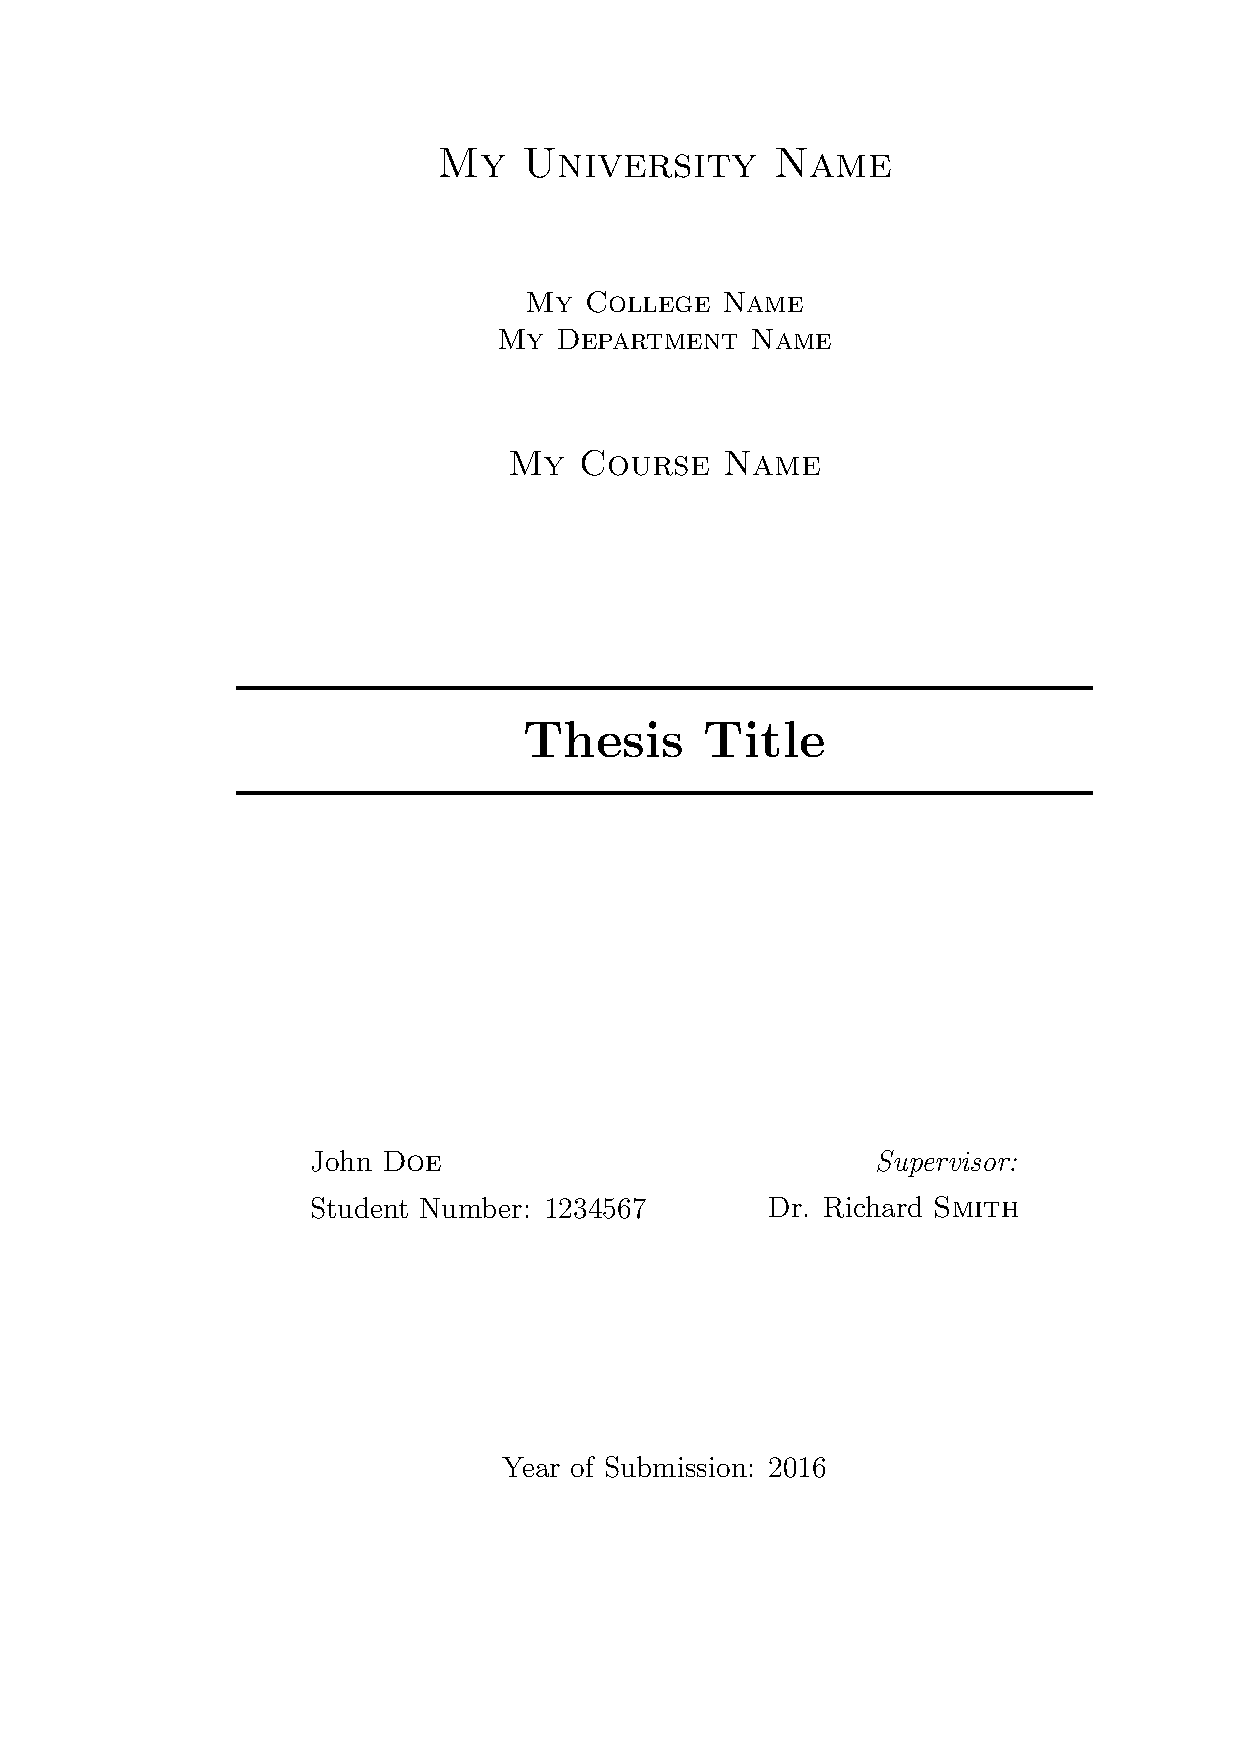
\includegraphics[width=.24\linewidth,page=1]{examples/fyp_example.pdf}
}
\fcolorbox{black}{white}{%
  \includegraphics[width=.24\linewidth,page=2]{examples/fyp_example.pdf}
}
\fcolorbox{black}{white}{%
  \includegraphics[width=.24\linewidth,page=3]{examples/fyp_example.pdf}
}
\fcolorbox{black}{white}{%
  \includegraphics[width=.24\linewidth,page=4]{examples/fyp_example.pdf}
}
\end{center}

\btVFill

\hfill\textsmaller{\LaTeX source available at \url{https://github.com/martinsbruveris/thesis-template}.} \\
\hfill\textsmaller{See also
\url{https://www.brunel.ac.uk/~mastmmb/mathwriting.html}.}

\medskip
\end{frame}

\begin{frame}
\frametitle{Highly Configurable Documents}
\framesubtitle{\texttt{memoir} and \textsmaller{KOMA}-Script Classes}

\begin{itemize}
\item Sectional headings
\item Running headers and footers
\item Good font, colour and illustration choices
\end{itemize}

%% See http://liantze.penguinattack.org/ebooks.html
\begin{center}
\onslide<2>{%
\fcolorbox{black}{white}{
\includegraphics[width=.24\linewidth,page=1]{examples/GridBookExcerpt}}
\fcolorbox{black}{white}{
\includegraphics[width=.24\linewidth,page=2]{examples/GridBookExcerpt}}
\fcolorbox{black}{white}{
\includegraphics[width=.24\linewidth,page=3]{examples/GridBookExcerpt}}
\fcolorbox{black}{white}{
\includegraphics[width=.24\linewidth,page=4]{examples/GridBookExcerpt}}
}
\end{center}
\end{frame}


\begin{frame}[fragile]
\frametitle{Presentation Slides}
\begin{itemize}
\item This presentation was made with \LaTeX.
\item<+-> Many possible classes: \texttt{powerdot}, \alert<2->{\texttt{beamer}}
\end{itemize}

\begin{columns}<+->
\begin{column}{.47\textwidth}
\begin{beamerboxesrounded}[width=\linewidth]{}
\vskip-1em
\begin{lstlisting}[basicstyle=\ttfamily\small,
moretexcs={usetheme,frametitle,frame,titleframe},
emph={beamer,frame},
escapechar={:},lineskip=-2pt]
\documentclass{beamer}
\usetheme{:\onslide<2>{\rlap{Warsaw\}}}%
\onslide<3|trans:0|handout:0>{\rlap{Szeged\}}}%
\onslide<4|trans:0|handout:0>{\rlap{Bergen\}}}%
\onslide<5|trans:0|handout:0>{\rlap{oxygen\}}}%
\onslide<6|trans:0|handout:0>{\rlap{Gelugor\}}}:

\author ...

\begin{document}
\titleframe

\section{Intro}

\begin{frame}
\frametitle{Some Background}
...
:\bfseries\color{Maroon}\textbackslash end:{frame}
\end{document}
\end{lstlisting}
\vspace*{-1em}
\end{beamerboxesrounded}
\end{column}
\begin{column}{.48\textwidth}
\centering
\onslide<2>{\fcolorbox{black}{white}{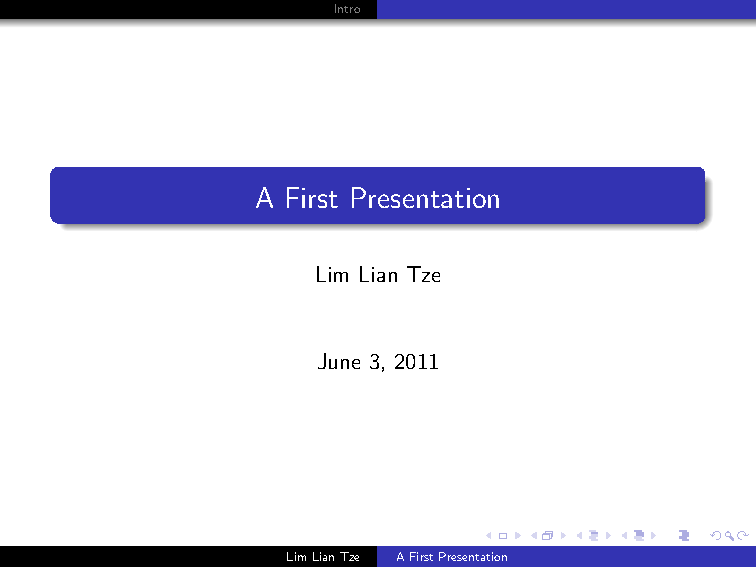
\includegraphics[width=.7\linewidth,page=1]{examples/beamer-Warsaw}}}%
\onslide<3|trans:0|handout:0>{\llap{\fcolorbox{black}{white}{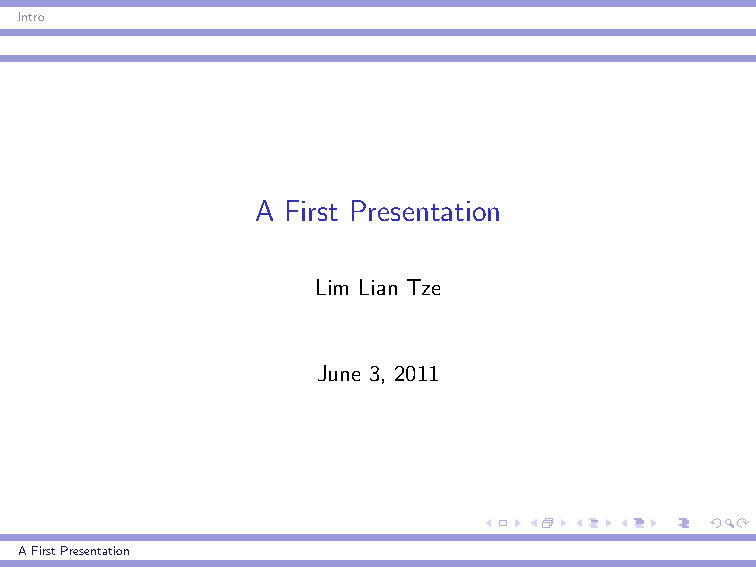
\includegraphics[width=.7\linewidth,page=1]{examples/beamer-Szeged}}
}}%
\onslide<4|trans:0|handout:0>{\llap{\fcolorbox{black}{white}{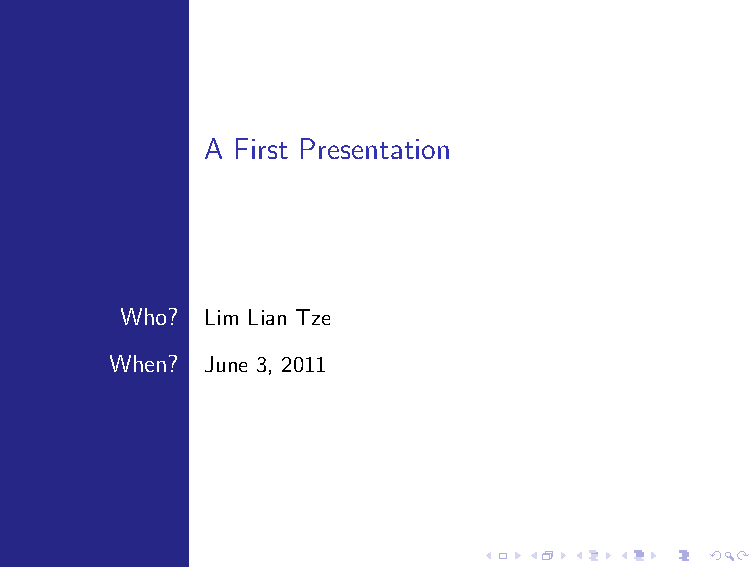
\includegraphics[width=.7\linewidth,page=1]{examples/beamer-Bergen}}
}}%
\onslide<5|trans:0|handout:0>{\llap{\fcolorbox{black}{white}{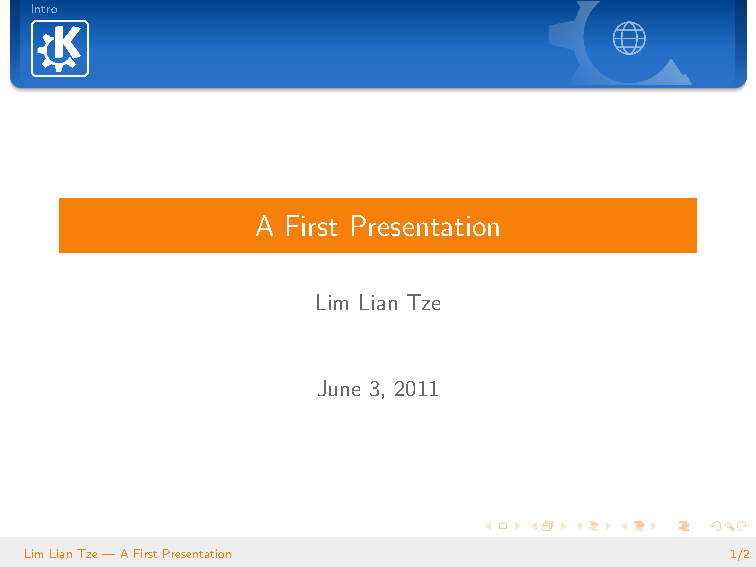
\includegraphics[width=.7\linewidth,page=1]{examples/beamer-Oxygen}}
}}%
\onslide<6|trans:0|handout:0>{\llap{\fcolorbox{black}{white}{
\includegraphics[width=.7\linewidth,page=1]{examples/beamer-Gelugor}}
}}
\onslide<2>{\fcolorbox{black}{white}{\includegraphics[width=.7\linewidth,page=2]{examples/beamer-Warsaw}}}%
\onslide<3|trans:0|handout:0>{\llap{\fcolorbox{black}{white}{\includegraphics[width=.7\linewidth,page=2]{examples/beamer-Szeged}}
}}%
\onslide<4|trans:0|handout:0>{\llap{\fcolorbox{black}{white}{\includegraphics[width=.7\linewidth,page=2]{examples/beamer-Bergen}}
}}%
\onslide<5|trans:0|handout:0>{\llap{\fcolorbox{black}{white}{\includegraphics[width=.7\linewidth,page=2]{examples/beamer-Oxygen}}
}}%
\onslide<6|trans:0|handout:0>{\llap{\fcolorbox{black}{white}{
\includegraphics[width=.7\linewidth,page=2]{examples/beamer-Gelugor}}
}}
\end{column}
\end{columns}
\end{frame}

\begin{frame}[fragile]
\frametitle{Oversized Posters}
\begin{itemize}
\item Many possible solutions:\\\texttt{sciposter}, \texttt{flowfram}, \texttt{beamerposter}, \texttt{tikzposter}
\end{itemize}

% beamerposter
\begin{columns}
\begin{column}{.5\textwidth}
\begin{beamerboxesrounded}[width=\linewidth]{}
\begin{lstlisting}[basicstyle=\ttfamily\small,
moretexcs={usetheme,frametitle,frame},
emph={beamer,beamerposter,frame},
escapechar={:},lineskip=-2pt]
\documentclass{beamer}
\usepackage[orientation=portrait, size=a0]{beamerposter}
\usetheme{...}
\author ... % Meta-information

\begin{document}
\begin{frame}
... % Poster contents goes here
:\bfseries\color{Maroon}\textbackslash end:{frame}
\end{document}
\end{lstlisting}
\end{beamerboxesrounded}
\end{column}
\begin{column}{.48\textwidth}
\centering
% See http://latex-my.blogspot.com/2011/03/creating-academic-posters-and-printing.html
\fcolorbox{black}{white}{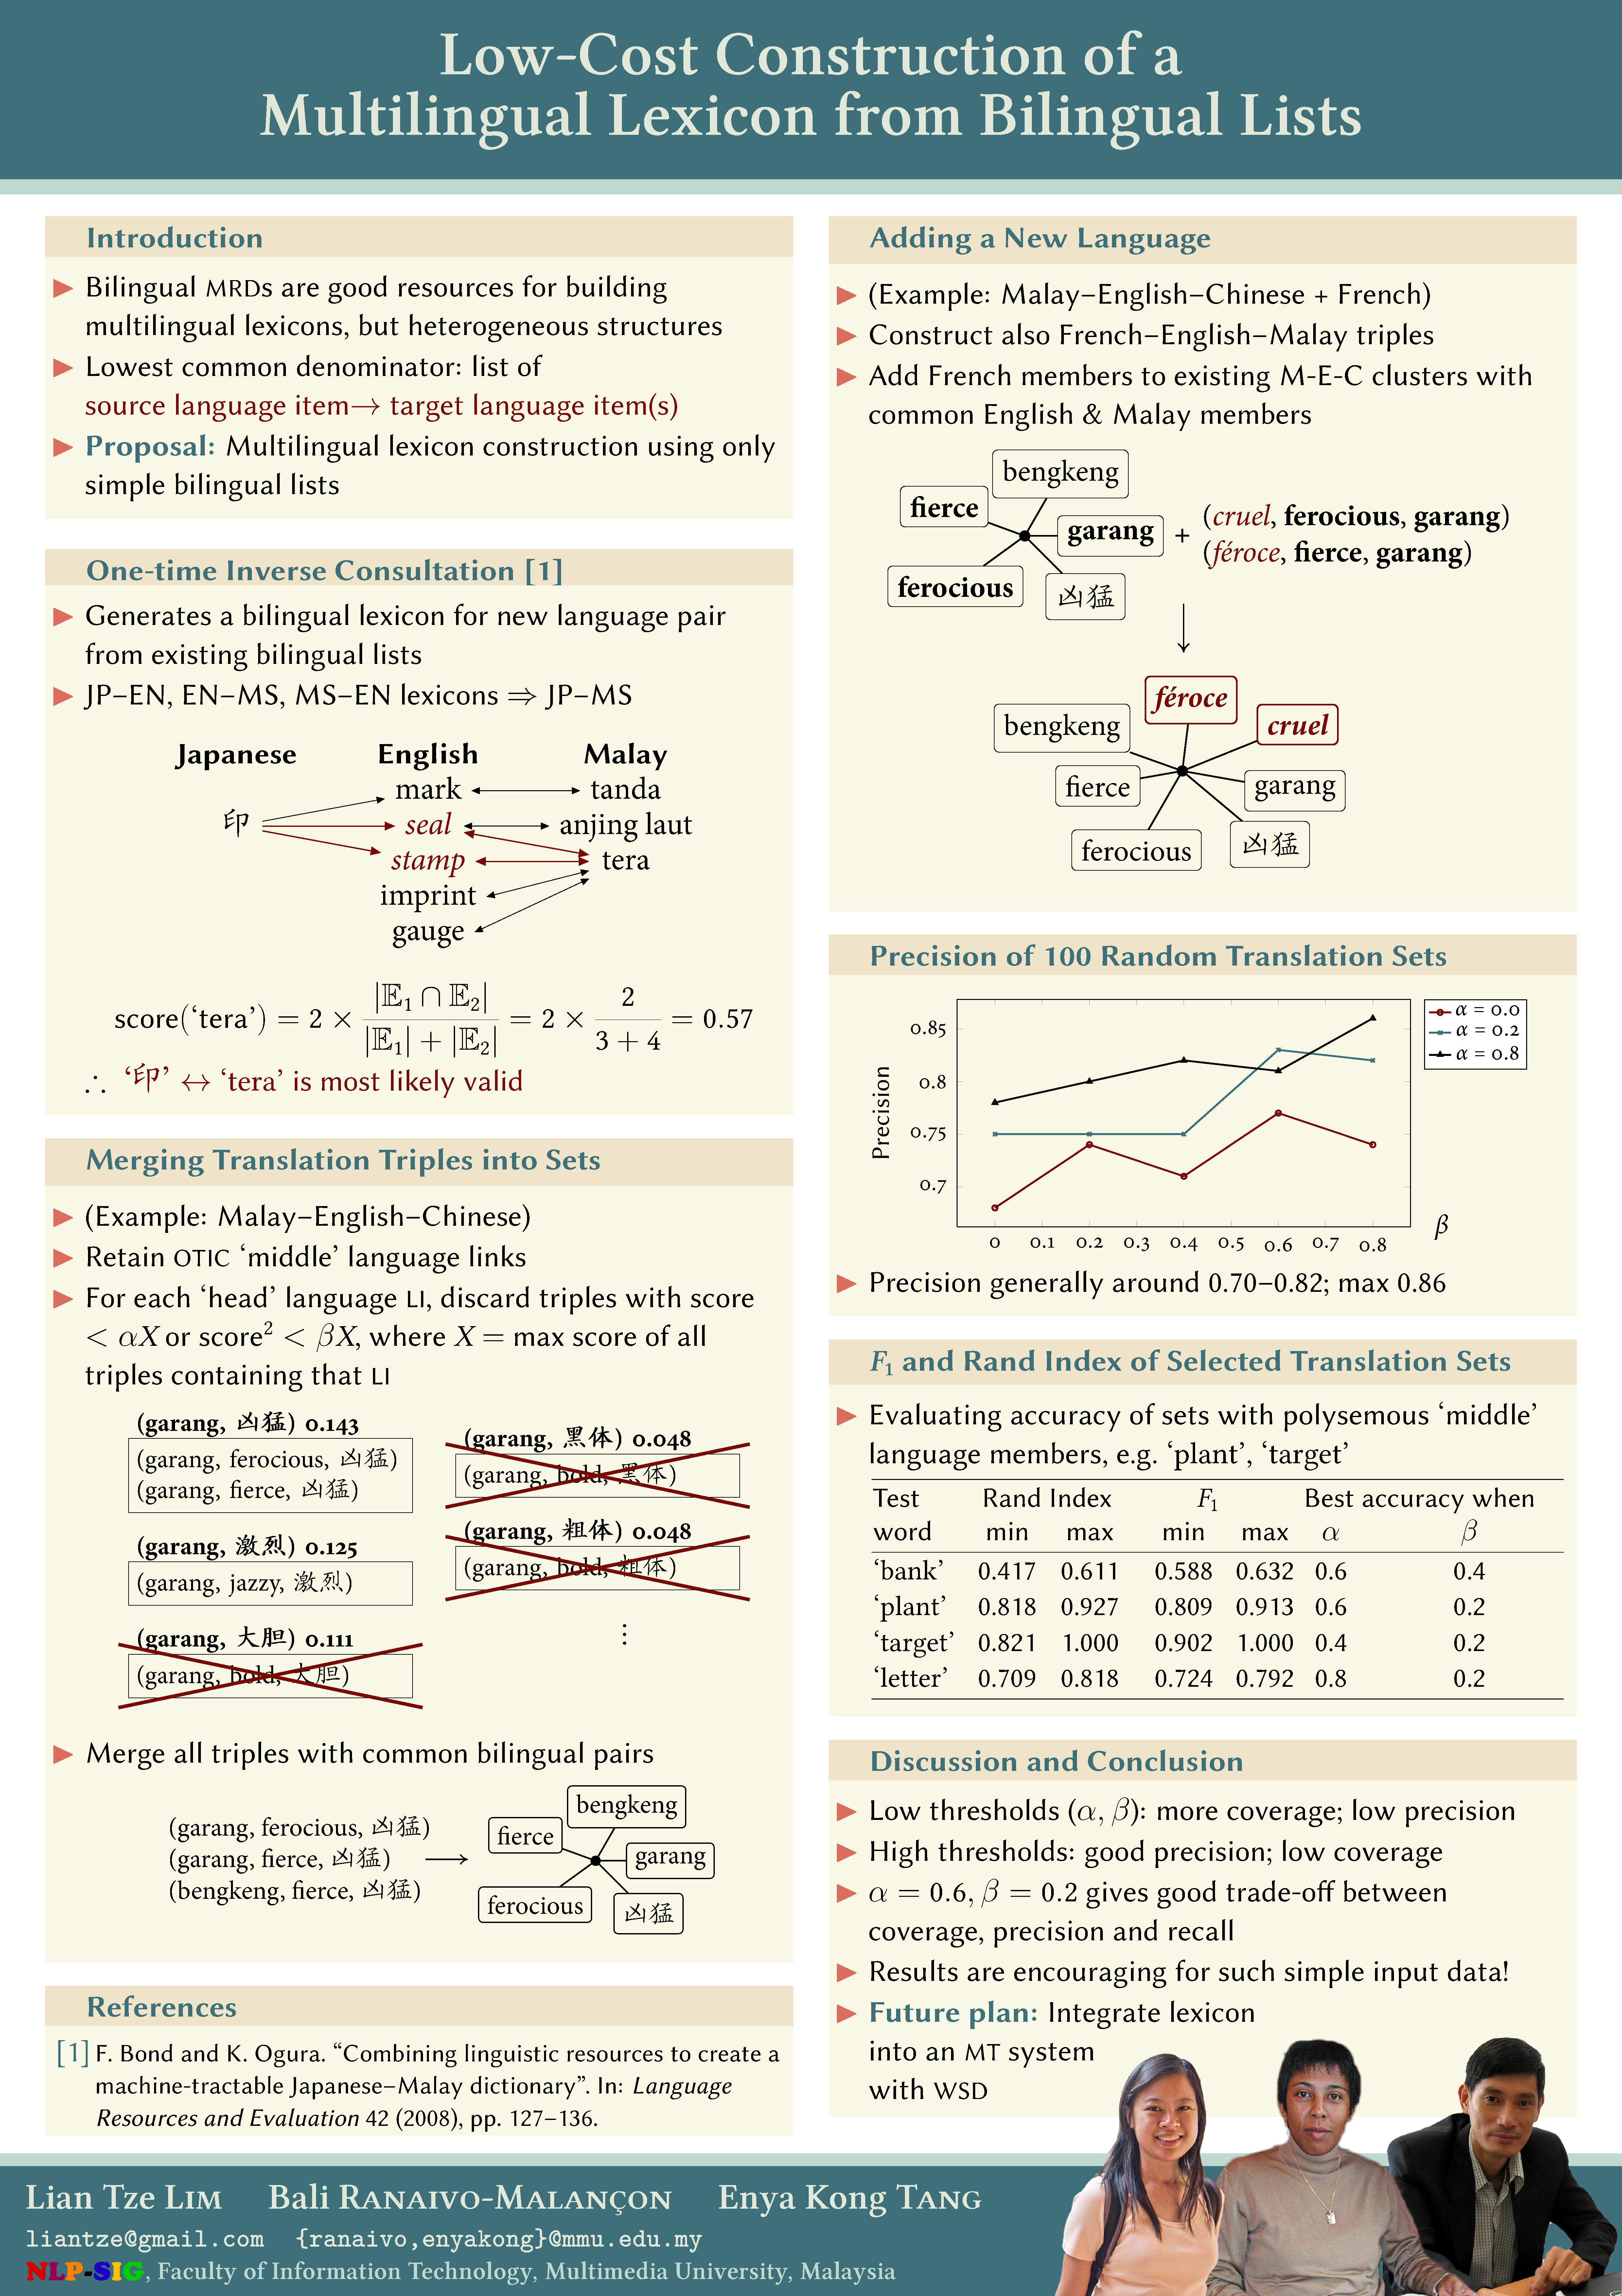
\includegraphics[width=.8\linewidth]{examples/cicling-poster-small.pdf}}
\end{column}
\end{columns}

\end{frame}

\begin{frame}[fragile]
\frametitle{Leaflets}

\texttt{leaflet} arranges contents into 6 pages on a foldable double-sided sheet.

\begin{columns}
\begin{column}{.496\textwidth}
\begin{beamerboxesrounded}[width=\linewidth]{}
\begin{lstlisting}[basicstyle=\ttfamily\small,lineskip=-2pt,emph={leaflet},moretexcs={maketitle}]
\documentclass[foldmark,a4paper]
{leaflet}
\author ... % Meta-information

\begin{document}
\maketitle
\section ...
... % Leaflet contents
\end{document}
\end{lstlisting}
\end{beamerboxesrounded}
\end{column}
\begin{column}{.48\textwidth}
\centering
% See http://latex-my.blogspot.com/2011/04/making-leaflets-with-l-t-e-x.html
\fcolorbox{black}{white}{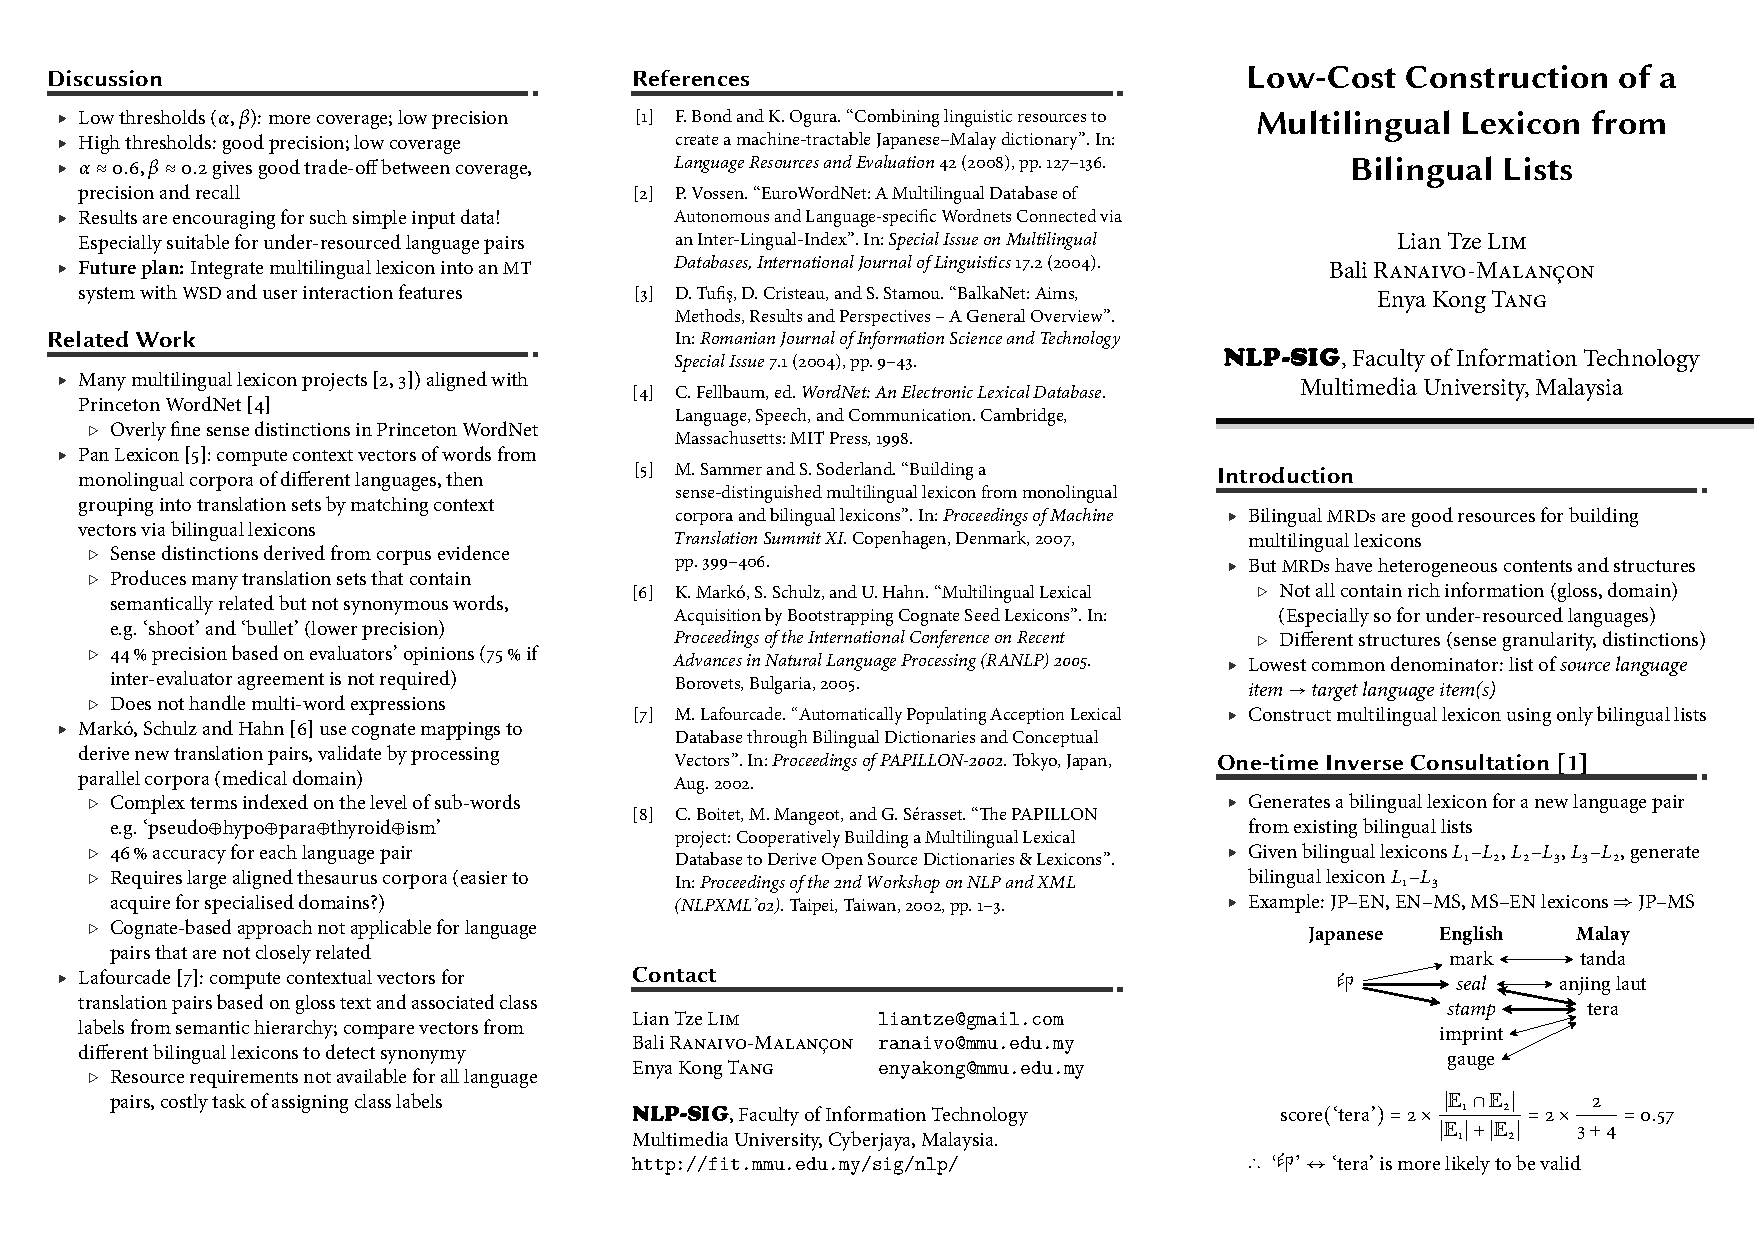
\includegraphics[width=.85\linewidth,page=1]{examples/cicling-handout.pdf}}
\fcolorbox{black}{white}{\includegraphics[width=.85\linewidth,page=2]{examples/cicling-handout.pdf}}\par
\end{column}
\end{columns}

\end{frame}


\begin{frame}[fragile]
\frametitle{Flash Cards}
\begin{columns}
\begin{column}{.47\textwidth}
\begin{beamerboxesrounded}{}
\vskip-1em
\begin{lstlisting}[basicstyle={\ttfamily\small},
emph={flashcards,flashcard},
moretexcs={cardfrontstyle,cardfrontfoot}]
\documentclass[avery5388,frame]
{flashcards}
\cardfrontstyle{headings}
\cardfrontfoot{Linux}

\begin{document}
\begin{flashcard}[Security]
{Certificate}
...
\end{flashcard}

\begin{flashcard}[Security]
{MAC ...}
...
\end{flashcard}
\end{document}
\end{lstlisting}
\vspace*{-1em}
\end{beamerboxesrounded}
\end{column}

\begin{column}{.53\textwidth}
\centering

\includegraphics[width=.49\linewidth,page=1]{examples/flashcard-crop}\hfill

\includegraphics[width=.49\linewidth,page=2]{examples/flashcard-crop}
\par
\end{column}
\end{columns}
\end{frame}


%%% Local Variables:
%%% TeX-master: "talk"
%%% End:
